%
% File rocling2026_draft.tex
% ROCLING 2026 短論文初稿（雙盲投稿版）
% 說明：所有【待補】處為實驗數據待填入位置；表格中 X.X 為佔位數字。
% 投稿前檢查：(1) \roclingfinalcopy 保持註解 (2) 全文無作者/機構資訊
%
\documentclass[11pt,a4paper]{article}
\usepackage[hyperref]{rocling2026}
\usepackage{times}
\usepackage{latexsym}
\usepackage{booktabs}
\usepackage{graphicx}
\renewcommand{\UrlFont}{\ttfamily\small}

% 中文字型設定（Overleaf 使用 XeLaTeX 編譯）
\usepackage{fontspec}
\usepackage{xeCJK}
\setCJKmonofont{AR PL UKai TW}
\setCJKmainfont{AR PL UKai TW}

\usepackage{microtype}

%\roclingfinalcopy % 投稿版保持註解（雙盲）；錄取後 camera-ready 才取消註解
%\def\roclingpaperid{***}

\newcommand\BibTeX{B\textsc{ib}\TeX}

\title{面向高齡語音互動應用之語音辨識部署方案比較：\\準確度、延遲與幻覺穩健性之權衡 \\
  Comparing ASR Deployment Options for Elderly Voice Interaction: \\ Trade-offs in Accuracy, Latency, and Hallucination Robustness}

% 雙盲投稿：保留作者欄空間但使用匿名占位
\author{Anonymous Author(s) \\
  Anonymous Affiliation \\
  Address line \\
  Address line \\
  \texttt{email@domain} \\}

\date{}

\begin{document}
\maketitle

\begin{abstractChinese}
語音互動平台是協助高齡者參與預立醫療照護計畫（Advance Care Planning, ACP）等健康決策的重要工具，其語音辨識（ASR）後端之選型須同時考量準確度、延遲、資源消耗、在地語言支援（繁體中文與台語），以及輸出之可靠性。本研究提出一個面向高齡語音互動場景之 ASR 部署評估框架，並在同一組測試條件下系統比較五種部署方案：雲端 Whisper large、本地端 Whisper small、加入語音活動偵測（VAD）門控之 Whisper、傳統 Kaldi 混合式系統，以及輕量串流模型 Nemotron 3.5 ASR 0.6B。除字元錯誤率（CER）與即時率（RTF）外，本研究特別納入「幻覺穩健性」評估：以自建之靜音、噪音、極短語音與猶豫音診斷集，量測各系統憑空生成文字與醫療關鍵詞幻覺之風險。實驗結果顯示【待補：主要發現一句話，如：端到端生成式模型在非語音輸入下幻覺率達 X\%，而 Kaldi 為 X\%；VAD 門控可將 Whisper 幻覺率降低 X\%】。本研究並據此提出高齡醫療語音應用之 ASR 部署決策建議。
\end{abstractChinese}

\begin{abstract}
Voice interaction platforms are increasingly used to support older adults in health decision-making tasks such as Advance Care Planning (ACP). Selecting an automatic speech recognition (ASR) backend for such applications requires balancing accuracy, latency, resource consumption, local language support (Traditional Chinese and Taiwanese Hokkien), and output reliability. This paper presents an evaluation framework for ASR deployment in elderly voice interaction scenarios and systematically compares five deployment profiles under identical test conditions: server-side Whisper large, on-device Whisper small, Whisper gated by voice activity detection (VAD), a conventional Kaldi hybrid system, and the lightweight streaming model Nemotron 3.5 ASR 0.6B. Beyond character error rate (CER) and real-time factor (RTF), we explicitly evaluate hallucination robustness using a purpose-built diagnostic set of silence, noise, very short utterances, and hesitation sounds, measuring both spurious text generation and hallucinated medical keywords. Results show that [TBD: key finding, e.g., end-to-end generative models hallucinate on X\% of non-speech inputs versus X\% for Kaldi, and VAD gating reduces Whisper hallucination by X\%]. We conclude with actionable deployment recommendations for elderly-facing medical voice applications.
\end{abstract}

\begin{keywordsChinese}
語音辨識、部署評估、幻覺、台語、高齡照護、預立醫療照護計畫
\end{keywordsChinese}

\begin{keywords}
Automatic Speech Recognition, Deployment Evaluation, Hallucination, Taiwanese Hokkien, Elderly Care, Advance Care Planning
\end{keywords}

\section{緒論}

台灣已進入超高齡社會，語音互動被視為協助高齡者跨越識能與數位落差的自然介面，近年亦逐漸應用於慢性病管理與健康決策支援等領域。預立醫療照護計畫（Advance Care Planning, ACP）是一個包含價值澄清、家庭討論與文件簽署之階段性歷程~\citep{schickedanz2009acp}；台灣高齡門診之調查顯示，非正式 ACP 討論雖普遍，正式意願文件之完成率仍偏低~\citep{lo2025acp}，顯示個人化決策輔助工具之需求。語音互動平台可以母語（國語與台語）引導高齡者理解醫療選項、澄清價值觀並提升行動準備度~\citep{sudore2017acp}。此類應用對語音辨識（Automatic Speech Recognition, ASR）後端提出了多重且彼此衝突的需求：辨識須準確、互動須即時、裝置端資源有限、須支援繁體中文與台語，且輸出必須可靠——在涉及生命末期意願的敏感對話中，辨識系統「憑空生成」使用者未曾說出的內容，其風險遠高於一般聽寫應用。

現行可選的 ASR 技術路線大致有三類。第一類為大型端到端多語模型，如 Whisper~\citep{radford2023whisper}，經社群微調後已可支援台灣華語繁體輸出與台語辨識，準確度高，但模型較大、串流延遲較高，且文獻已指出其在靜音與噪音輸入下存在幻覺（hallucination）現象~\citep{koenecke2024careless,frieske2024hallucination}。第二類為傳統混合式（hybrid）系統，如 Kaldi~\citep{povey2011kaldi}，其解碼受聲學模型與語言模型之詞圖（lattice）約束，原則上不會生成訓練詞表外的長段虛構內容，輸出行為可控，但建置與維護成本較高。第三類為新興輕量串流模型，如 NVIDIA Nemotron 3.5 ASR 0.6B~\citep{nvidia2026nemotron}，以 0.6B 參數達成 CPU 即時串流辨識，適合邊緣部署，惟其華語僅支援簡體輸出，且不支援台語，須仰賴簡繁轉換後處理，並面臨一簡對多繁之歧義風險。

既有 ASR 評測多聚焦於單一維度的字錯誤率比較，較少針對「高齡醫療語音互動」此一交叉場景，同時考量準確度、延遲、在地語言支援與輸出穩健性之部署層級比較；納入幻覺穩健性作為部署選型指標的實證研究更為罕見。本研究以一個實際開發中的高齡 ACP 語音互動平台為目標場景，提出部署評估框架並回答以下研究問題：

\begin{itemize}
  \item RQ1：在繁體中文與台語測試條件下，各部署方案之準確度與延遲/資源權衡為何？
  \item RQ2：在靜音、噪音、極短語音等非典型輸入下，各系統之幻覺風險有多大？是否會憑空生成醫療關鍵詞？
  \item RQ3：簡單之工程緩解手段（如 VAD 門控）能否使生成式模型達到接近傳統系統之穩健性？
\end{itemize}

本研究之貢獻有三：(1) 提出面向高齡語音互動之五維度 ASR 部署評估框架（準確度、延遲與資源、語言覆蓋、幻覺穩健性、可部署性）；(2) 建立包含靜音、噪音、極短語音、猶豫音與 ACP 關鍵詞句之幻覺診斷測試集，並完成五種部署方案之系統性實證比較；(3) 據實驗結果提出高齡醫療語音應用之 ASR 部署決策建議。

\section{相關研究}

\subsection{ASR 模型與部署路線}

Whisper~\citep{radford2023whisper} 以大規模弱監督訓練取得跨語言之強健辨識能力，為目前繁體中文與台語應用之主流基礎模型；透過微調可進一步提升台灣華語與台語表現~\citep{liao2020tat}。傳統混合式系統以 Kaldi~\citep{povey2011kaldi} 為代表，結合聲學模型、發音詞典與 n-gram 語言模型，解碼過程受詞圖約束。近年輕量串流模型快速發展，FastConformer~\citep{rekesh2023fastconformer} 搭配 RNN-T 解碼器~\citep{graves2012rnnt} 之 cache-aware 串流架構，使 0.6B 等級模型可於 CPU 達成低延遲即時辨識；Nemotron 3.5 ASR~\citep{nvidia2026nemotron} 以單一模型支援 40 種語言變體，惟華語僅列簡體（zh-CN）。上述三類路線在準確度、延遲與可控性上各有取捨，然而少有研究將其置於同一應用場景下進行部署層級之比較。

\subsection{ASR 幻覺}

端到端生成式 ASR 的解碼本質上是條件式文字生成，在輸入訊號資訊不足（靜音、噪音、極短語音）時，模型可能輸出與輸入無關之流暢文句。\citet{koenecke2024careless} 分析 Whisper 之轉錄輸出，發現約 1\% 之音檔出現整句幻覺，其中近四成內容具潛在危害性，且對特定語者族群（如言語障礙者）更為嚴重；\citet{frieske2024hallucination} 則提出以噪音注入評估 ASR 幻覺傾向之方法。於醫療對話場景，幻覺可能將使用者之猶豫或沉默誤轉為具體之醫療意願陳述，構成臨床風險。然而，現有 ASR 選型與評測實務多未將幻覺穩健性納入標準指標，本研究將其明確納入部署評估框架。

\subsection{高齡語音應用與台語 ASR}

語音介面特別適合視力退化、識能不足或不熟悉科技之高齡族群，近年於慢性病自我管理與高齡照護輔助之應用漸增。於台灣情境，台語為高齡族群之主要生活語言，台語 ASR 資源以 TAT 語料庫~\citep{liao2020tat} 等為代表；繁體中文評測則常用 Common Voice~\citep{ardila2020commonvoice} 之 zh-TW 子集。本研究以 ACP 語音互動平台為目標場景：該類平台須以國台語雙語引導高齡者進行價值澄清與醫療偏好表達~\citep{sudore2017acp}，且面向多元識能背景之高齡使用者的數位健康工具，須經迭代設計以降低使用與理解負擔~\citep{scheerens2021ehealth}，對 ASR 之語言覆蓋與輸出可靠性均有嚴格要求。

\section{研究方法}

\subsection{部署方案定義}

本研究比較表~\ref{tab:profiles} 所列之五種部署方案（deployment profiles）。方案之選取涵蓋三類技術路線與兩種部署位置：D1 代表雲端高準確度上限；D2 代表本地端可離線之平衡方案；D3 在 D2 之上加入語音活動偵測（Voice Activity Detection, VAD）門控，僅於偵測到語音時送入辨識器，作為幻覺之工程緩解手段~\citep{silero2021vad}；D4 為傳統混合式系統，代表輸出可控之穩健路線；D5 為輕量串流模型，因其僅輸出簡體中文，附加 OpenCC~\citep{opencc} 之 s2twp 組態進行簡繁轉換後處理。D5 不支援台語，於台語測試中標記為不適用（N/A），此一語言覆蓋限制本身即為部署比較之重要結果。

\begin{table*}[t]
\centering
\small
\begin{tabular}{llllll}
\toprule
\textbf{編號} & \textbf{引擎} & \textbf{部署位置} & \textbf{串流} & \textbf{語言覆蓋} & \textbf{後處理} \\
\midrule
D1 & Whisper large-v3 & GPU 伺服器 & 否 & 繁中＋台語 & 無 \\
D2 & Whisper small & 本地 CPU/GPU & 否 & 繁中＋台語 & 無 \\
D3 & Whisper small + VAD & 本地 CPU/GPU & 否 & 繁中＋台語 & VAD 門控 \\
D4 & Kaldi 混合式系統 & 本地 CPU & 是 & 繁中＋台語 & 自定義詞表 \\
D5 & Nemotron 3.5 ASR 0.6B & 本地 CPU & 是（80ms） & 簡體國語 & OpenCC s2twp \\
\bottomrule
\end{tabular}
\caption{\label{tab:profiles} 本研究比較之五種 ASR 部署方案。【待補：依實際使用之模型版本與 Kaldi 系統組態修訂】}
\end{table*}

\subsection{評估框架}

本研究自高齡語音互動應用之實際需求出發，定義五個評估維度：

\begin{enumerate}
  \item \textbf{準確度}：一般語句之字元錯誤率（CER），以及 ACP 醫療關鍵詞（如「預立醫療決定」、「心肺復甦術」、「醫療委任代理人」）之關鍵詞錯誤率。
  \item \textbf{延遲與資源}：即時率（Real-Time Factor, RTF）、端到端延遲、峰值記憶體與模型大小，於 CPU 與 GPU 環境各別量測。
  \item \textbf{語言覆蓋}：是否原生支援繁體中文輸出與台語辨識，或須仰賴後處理。
  \item \textbf{幻覺穩健性}：非語音或退化輸入下憑空生成文字之傾向（3.3 節）。
  \item \textbf{可部署性}：是否可離線執行、是否支援串流、與行動應用整合之工程成本（定性分析）。
\end{enumerate}

\subsection{幻覺診斷測試集}

高齡者於 ACP 對話中常出現長時間停頓、猶豫與極短回應，此類輸入正是生成式 ASR 最易產生幻覺之條件。本研究建構幻覺診斷測試集，共【待補：實際段數】段音訊，包含五種條件：(1) 純靜音（3--10 秒，20 段）；(2) 環境噪音（病房背景、電扇、街道，20 段）；(3) 極短語音（1--3 字之真實語音，20 段）；(4) 猶豫音（「嗯」、「啊」等填充音，20 段）；(5) 正常 ACP 語句（對照組，計算 CER，【待補】段）。

對每一段輸入，記錄三項指標：(a) \textbf{幻覺率}：輸出非空文字之比例（條件 1、2）；(b) \textbf{平均插入字數}：輸出字數超出參考轉錄之插入量（條件 3、4）；(c) \textbf{關鍵詞幻覺}：輸出中憑空出現 ACP 醫療關鍵詞之次數。其中關鍵詞幻覺為本場景最具臨床意義之風險指標：若系統於使用者沉默時輸出「不要急救」等內容，將直接汙染下游對話狀態追蹤與意願紀錄。

\section{實驗設定}

\subsection{測試資料}

國語測試採用 Common Voice~\citep{ardila2020commonvoice} zh-TW 測試集【待補：版本與抽樣句數】；台語測試採用【待補：TAT 子集或實驗室測試集之描述，注意匿名化】~\citep{liao2020tat}。ACP 關鍵詞句由研究團隊參考預立醫療照護諮商實務編寫【待補：句數】句，由【待補：錄音者描述，如多名成年語者以國語與台語錄製】。幻覺診斷集依 3.3 節設計錄製與剪輯。所有測試資料之取樣率統一為 16 kHz。

\subsection{系統實作細節}

D1、D2 使用【待補：whisper 實作，如 faster-whisper vX.X】；繁體中文與台語辨識採用【待補：微調模型或 prompt 設定之匿名描述】。D3 之 VAD 採用 Silero VAD~\citep{silero2021vad}，門檻設為【待補】。D4 之 Kaldi 系統為【待補：聲學模型架構（如 TDNN chain model）、語言模型與詞典規模之描述】。D5 使用 NVIDIA NeMo 框架載入 nemotron-3.5-asr-streaming-0.6b 官方檢查點，語言提示設為 zh-CN，輸出經 OpenCC s2twp 轉換為台灣正體。

\subsection{硬體與量測}

伺服器端實驗於【待補：GPU 型號】執行；本地端實驗於【待補：CPU 型號、核心數、記憶體】執行，模擬平板/迷你主機等場域裝置之資源條件。RTF 以總解碼時間除以音訊長度計算，重複三次取平均。延遲量測【待補：量測方式，串流系統另報首字延遲】。

\section{實驗結果與討論}

\subsection{準確度與效能（RQ1）}

表~\ref{tab:main} 為各部署方案於國語、台語測試集之 CER、ACP 關鍵詞錯誤率與效能指標。

\begin{table*}[t]
\centering
\small
\begin{tabular}{lcccccc}
\toprule
\textbf{方案} & \textbf{國語 CER (\%)} & \textbf{台語 CER (\%)} & \textbf{關鍵詞錯誤率 (\%)} & \textbf{RTF (CPU)} & \textbf{延遲 (s)} & \textbf{記憶體 (GB)} \\
\midrule
D1 Whisper large   & X.X & X.X & X.X & X.X & X.X & X.X \\
D2 Whisper small   & X.X & X.X & X.X & X.X & X.X & X.X \\
D3 Whisper + VAD   & X.X & X.X & X.X & X.X & X.X & X.X \\
D4 Kaldi           & X.X & X.X & X.X & X.X & X.X & X.X \\
D5 Nemotron + 轉繁 & X.X & N/A & X.X & X.X & X.X & X.X \\
\bottomrule
\end{tabular}
\caption{\label{tab:main} 各部署方案之準確度與效能總表。【待補：全部數據；台語欄 D5 為 N/A 係因該模型不支援台語】}
\end{table*}

【待補：結果敘述段落。建議涵蓋：(1) D1 與 D2 之 CER 差距與資源代價；(2) D4 相對 Whisper 之準確度落差是否在可接受範圍；(3) D5 於國語之 CER、經 OpenCC 轉繁後之殘留簡繁錯誤（如一簡對多繁錯例），以及其 RTF/延遲優勢之量化；(4) 台語欄位顯示之語言覆蓋差異。】

圖~\ref{fig:tradeoff} 以準確度—延遲散點圖呈現整體權衡，點之大小表示幻覺率。【待補：matplotlib 產出 tradeoff.pdf 後取消下方註解】

\begin{figure}[t]
\centering
% 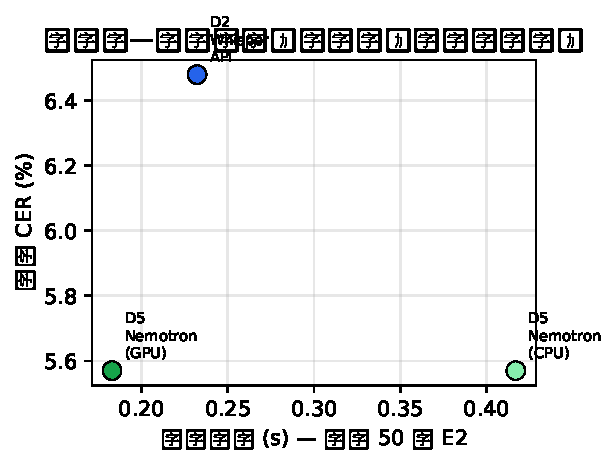
\includegraphics[width=\columnwidth]{tradeoff.pdf}
\fbox{\parbox{0.9\columnwidth}{\centering\vspace{2cm}【待補：圖 1 準確度—延遲權衡圖\\（x 軸：延遲或 RTF；y 軸：CER；\\點大小/顏色：幻覺率）】\vspace{2cm}}}
\caption{\label{fig:tradeoff} 各部署方案之準確度—延遲權衡（點大小表示非語音輸入之幻覺率）。}
\end{figure}

\subsection{幻覺穩健性（RQ2）}

表~\ref{tab:halluc} 為幻覺診斷集之結果。

\begin{table}[t]
\centering
\small
\begin{tabular}{lccc}
\toprule
\textbf{方案} & \textbf{幻覺率 (\%)} & \textbf{插入字數} & \textbf{關鍵詞幻覺} \\
\midrule
D1 & X.X & X.X & X \\
D2 & X.X & X.X & X \\
D3 & X.X & X.X & X \\
D4 & X.X & X.X & X \\
D5 & X.X & X.X & X \\
\bottomrule
\end{tabular}
\caption{\label{tab:halluc} 幻覺診斷集結果：幻覺率（靜音＋噪音條件下輸出非空文字之比例）、平均插入字數（極短語音與猶豫音條件），與 ACP 關鍵詞幻覺總次數。【待補】}
\end{table}

【待補：結果敘述段落。建議涵蓋：(1) Whisper 系列於靜音/噪音下之幻覺率與典型錯例（引述實際輸出句）；(2) Kaldi 於相同條件下之行為（預期為空輸出或零星單字，驗證「詞圖約束、不易幻覺」之假設）；(3) Nemotron 之幻覺行為（RNN-T 相較 attention-based encoder-decoder 之差異）；(4) 是否觀察到關鍵詞幻覺及其臨床意涵。】

\subsection{VAD 門控之緩解效果（RQ3）}

【待補：比較 D2 與 D3。建議涵蓋：(1) VAD 門控使幻覺率自 X\% 降至 X\%；(2) 對正常語句 CER 之影響（是否誤切導致 CER 上升）；(3) 對延遲之額外開銷；(4) 結論：VAD 門控後之 Whisper 能否達到接近 D4 之穩健性，同時保留多語優勢。】

\subsection{錯誤分析}

【待補：質性錯例分析。建議以小表或行內引述呈現 2--4 個代表性錯例：(1) Whisper 靜音幻覺輸出之完整句；(2) D5 經 OpenCC 後殘留之一簡對多繁錯誤（如「頭髮/頭發」、「後面/后面」類）；(3) 台語語句於各系統之輸出差異；(4) 高齡語速/猶豫語音之辨識行為。】

\subsection{部署建議}

綜合上述結果，表~\ref{tab:decision} 給出面向高齡醫療語音應用之部署決策建議。【待補：依實際結果修訂下表內容與敘述】

\begin{table}[t]
\centering
\small
\begin{tabular}{p{0.44\columnwidth}p{0.44\columnwidth}}
\toprule
\textbf{應用場景} & \textbf{建議方案} \\
\midrule
國台語雙語、準確度優先、可用伺服器 & D1（Whisper large） \\
本地離線、一般衛教互動 & D3（Whisper + VAD） \\
敏感意願對話、輸出須可控 & D4（Kaldi）或 D3 搭配確認機制 \\
極低延遲串流、僅國語、可容忍簡繁後處理 & D5（需審慎評估） \\
台語使用者 & D1--D4（D5 不適用） \\
\bottomrule
\end{tabular}
\caption{\label{tab:decision} 高齡醫療語音應用之 ASR 部署決策建議。}
\end{table}

\section{結論與未來工作}

本研究針對高齡語音互動應用，提出納入幻覺穩健性之五維度 ASR 部署評估框架，並對五種部署方案完成系統性實證比較。結果顯示【待補：三點主要結論之一句話總結：(1) 準確度—延遲權衡；(2) 幻覺風險差異與 VAD 緩解效果；(3) 輕量模型之在地語言覆蓋缺口】。本研究之主要意涵為：於醫療敏感場景之 ASR 選型，輸出穩健性應與字錯誤率並列為第一級指標。

未來工作包括：(1) 擴大高齡真實語者之測試規模，納入語速、構音與方言變異之分析；(2) 探索輕量串流模型之繁體中文與台語適配（詞表擴充與低資源微調）；(3) 將本框架之量測整合至語音互動平台之持續評估流程，並於實際場域驗證幻覺緩解機制對下游對話品質之影響。

% 投稿版不可包含致謝
%\section*{Acknowledgments}

\bibliography{rocling2026}
\bibliographystyle{acl_natbib}

\end{document}
